% !TEX program = pdflatex
% =============================================================================
% REDIN article — Final Henry (Agamaz + adaptive inference)
% Adapted for REDIN: single column, letter paper, 12pt, line numbers
% Compile: pdflatex article_REDIN.tex  (twice)
% =============================================================================
\documentclass[12pt,letterpaper]{article}

% --- Fonts (pdfLaTeX, Times-like; reliable on TeX Live) ---
\usepackage[T1]{fontenc}
\usepackage[utf8]{inputenc}
\usepackage{mathptmx}
\usepackage[scaled=0.92]{helvet}
\usepackage{courier}

% --- Language ---
\usepackage[spanish,es-tabla,english]{babel}
% --- Math / symbols ---
\usepackage{amsmath,amssymb,amsfonts}
\usepackage{textcomp}
\usepackage{microtype}

% --- Graphics ---
\usepackage{graphicx}
% Resolve only the curated figures directory: avoids stale duplicates in paper/.
\graphicspath{{figures/}}
\usepackage[font={normalsize},labelfont=md,skip=6pt]{caption}
\usepackage{subcaption}

% --- Tables ---
\usepackage{booktabs}
\usepackage{array}
\usepackage{tabularx}
\usepackage{multirow}
\usepackage{makecell}
\usepackage{siunitx}
\sisetup{detect-all, group-separator={,}, group-minimum-digits=4}

% --- Layout ---
\usepackage[margin=2.5cm]{geometry}
\usepackage{setspace}
\setstretch{1.0}
\usepackage{titlesec}
\titleformat{\section}{\normalfont\Large\bfseries}{\thesection.}{0.5em}{}
\titleformat{\subsection}{\normalfont\large\bfseries}{\thesubsection.}{0.4em}{}
\titlespacing*{\section}{0pt}{12pt plus 2pt}{6pt plus 1pt}
\titlespacing*{\subsection}{0pt}{10pt plus 1pt}{4pt plus 1pt}

% --- Refs / links (hyperref last) ---
\usepackage[numbers,sort&compress]{natbib}
\usepackage[colorlinks=true,linkcolor=black,citecolor=blue,urlcolor=blue]{hyperref}

% --- Authors ---
\usepackage{authblk}
\renewcommand\Authfont{\normalsize}
\renewcommand\Affilfont{\small\itshape}

% --- Line numbers (REDIN requirement) ---
\usepackage{lineno}

\usepackage{placeins}

% Keep figures in the text flow: allow a tall figure at the top of a text page.
\renewcommand{\topfraction}{0.90}
\renewcommand{\textfraction}{0.10}
\renewcommand{\floatpagefraction}{0.80}
\setcounter{topnumber}{3}
\setcounter{totalnumber}{5}

\hypersetup{
  pdftitle={Multiscale Heterogeneity of an Urban PM2.5 Monitoring Network: Wavelet-Based Functional Inference for Lima, Peru},
  pdfauthor={Henry S. Aquino-Mosquera; Jaime E. Villanueva-Ram\'irez; Daniel A. Huam\'an-C\'ardenas; Gualberto R. Quispe-Mendoza},
  pdfkeywords={wavelet transform; PM2.5; multiscale analysis; functional ANOVA; air quality monitoring}
}

\begin{document}
\linenumbers

% ═══════════════════════════════════════════════════════════
\title{Multiscale Heterogeneity of an Urban PM2.5\\
Monitoring Network: Wavelet-Based Functional Inference for Lima, Peru\\[0.55em]
\large Heterogeneidad multiescala de una red urbana de monitoreo de PM2.5:\\
inferencia funcional wavelet para Lima, Per\'u}

\author[1]{Henry S. Aquino-Mosquera}
\author[2]{Jaime E. Villanueva-Ram\'irez}
\author[3]{Daniel A. Huam\'an-C\'ardenas}
\author[4]{Gualberto R. Quispe-Mendoza}

\affil[1]{Departamento de Matem\'atica Aplicada, Universidad Andina de Ciencias y Tecnolog\'ia, Av. Universitaria 450, Lima 15023, Per\'u}
\affil[2]{Laboratorio de Monitoreo Atmosf\'erico, Instituto de Ingenier\'ia Ambiental del Per\'u, Jr. Las Flores 128, San Isidro, Lima 15073, Per\'u}
\affil[3]{Escuela de Estad\'istica, Universidad Nacional de Ingenier\'ia, Av. T\'upac Amaru 210, R\'imac, Lima 15333, Per\'u}
\affil[4]{Unidad de An\'alisis Multiescala, Centro de Estudios Estad\'isticos Avanzados, Calle Schell 343, Miraflores, Lima 15074, Per\'u}

\date{}
\maketitle

% ── ABSTRACT ──────────────────────────────────────────────
\selectlanguage{english}
\renewcommand{\abstractname}{Abstract}
\begin{abstract}
\noindent
Urban PM2.5 networks are evaluated through mean concentrations or exceedance counts, which cannot reveal when stations behave differently. We analyse hourly PM2.5 at five REMCA stations in Lima, Peru (1~January 2022--28~February 2023; $n=10{,}176$) with a wavelet framework combining conservative preprocessing and assumption-checked inference. Missing values were interpolated per station (2.4--6.8\%). Isolated instrumental errors were replaced only when two residual rules flagged them and no other station corroborated them (69--110~h per station; 0.68--1.08\%), compared with 8--13\% under STL+$3\times$IQR. A Symmlet-7 wavelet transform on mirror-padded series ($2^{14}$) supported tests on central coefficients at $j=1,\ldots,9$ (Bonferroni $M=9$) using repeated-measures ANOVA, Friedman, or block-permutation tests ($N_{\mathrm{perm}}=9{,}999$). Bonferroni-significant differences occur at $j=1$--$7$, peak in the diurnal band $j=4$ (Kendall's $W=0.69$), and lose Bonferroni support at $j=8$; no evidence of a difference at $j=9$, and $j\ge 10$ was not formally testable. Diurnal energy is 20.4\% at San Juan de Lurigancho versus 12.4\% at San Borja. Sensitivity preserves the $j=1$--$7$ pattern. The results support denser short-scale coverage in high-contrast corridors and caution against treating multi-week signals as station-specific.

\medskip
\noindent\textbf{Keywords:}
wavelet transform; PM2.5; multiscale analysis; functional ANOVA; air quality monitoring.
\end{abstract}

\vspace{0.4em}
\noindent\rule{\textwidth}{0.4pt}
\vspace{0.3em}

% ── RESUMEN ───────────────────────────────────────────────
\selectlanguage{spanish}
\noindent\textbf{Resumen.}
Las redes de PM2.5 suelen evaluarse mediante concentraciones medias o recuentos de superaciones, que no revelan cu\'ando las estaciones se comportan de forma distinta. Analizamos PM2.5 horario en cinco estaciones REMCA de Lima (1~enero~2022--28~febrero~2023; $n=10{,}176$) con un enfoque wavelet multiescala que combina preprocesamiento conservador e inferencia condicionada a diagn\'osticos. Se imputaron los valores faltantes por estaci\'on (2{,}4--6{,}8\%) y solo se sustituyeron errores instrumentales aislados cuando dos reglas de residuos los se\~nalaron y ninguna otra estaci\'on los corrobor\'o (69--110~h; 0{,}68--1{,}08\%), frente al 8--13\% de STL+$3\times$IQR. Con DWT Symmlet-7 y pruebas en $j=1,\ldots,9$ (Bonferroni $M=9$; $N_{\mathrm{perm}}=9{,}999$), las diferencias son significativas en $j=1$--$7$, m\'aximas en la banda diurna $j=4$ ($W=0{,}69$) y dejan de serlo tras la correcci\'on de Bonferroni en $j=8$; no hay evidencia de diferencia en $j=9$ y $j\ge10$ no pudo evaluarse formalmente. La energ\'ia diurna es 20{,}4\% en SJL y 12{,}4\% en SBJ. Los an\'alisis de sensibilidad conservan el patr\'on. Los resultados apoyan una mayor cobertura en escalas cortas en corredores contrastados y cautela al interpretar se\~nales de varias semanas como espec\'ificas de estaci\'on.

\medskip
\noindent\textbf{Palabras clave:}
transformada wavelet; PM2.5; an\'alisis multiescala; ANOVA funcional; monitoreo de calidad del aire.

\noindent\rule{\textwidth}{0.4pt}
\vspace{0.5em}
\selectlanguage{english}

% =============================================================================
\section{Introduction}
\label{sec:intro}
% =============================================================================

Fine particulate matter (PM2.5) is a leading environmental risk factor for urban public health. In Peru, ambient PM2.5 is associated with approximately 230 premature deaths per million inhabitants, among the highest rates in the Americas~\cite{watts2018}. Metropolitan Lima has long ranked among the most polluted large cities in Latin America for particulate matter~\cite{iqair2023}, with multi-station analyses documenting persistent exceedances of national and World Health Organization (WHO) guidelines and strong spatial contrasts across northern, eastern and southern districts~\cite{pacsi2016,campos2024,vu2019,who2021}. Lima faces recurrent wintertime deterioration driven by traffic and industrial emissions and by meteorological regimes that suppress vertical mixing~\cite{pacsi2016,campos2024}.

The Peruvian National Service of Meteorology and Hydrology (SENAMHI) operates the Air Quality Monitoring Network (REMCA, Red de Monitoreo de Calidad del Aire), which records hourly PM2.5 at stations distributed across the metropolitan area. Exposure-mapping and network studies in Lima show that sparse monitors and strong intra-urban gradients make station placement and redundancy non-trivial design questions~\cite{vu2019,romerobaylon2024}. Operational analyses often reduce these series to daily means, exceedance counts, or classical ANOVA on scalars. Such summaries are sensitive to outliers and right skew, and---more importantly---they cannot locate the \emph{timescales} of spatial heterogeneity~\cite{morettin2017,ignaccolo2008}. Functional data analysis treats each station as a curve rather than a single number~\cite{cardot1999,hall2007}. Wavelet bases further localise differences jointly in scale and time~\cite{abramovich2000,antoniadis2007}, and have been used to characterise monitoring-site similarity and local-versus-background variability in air-quality networks~\cite{gouveia2015,zimmerman2020}. Wavelet-based functional ANOVA (wavelet-FANOVA) projects curves onto detail coefficients so that scale-wise tests can be stated in finite dimension~\cite{abramovich2006,ma2018}. What remains missing for Lima is a scale-resolved assessment of whether stations are redundant for specific monitoring objectives, rather than only whether their marginal distributions differ.

Two methodological difficulties arise with environmental series. First, aggressive residual fences (e.g.\ STL+$3\times$IQR, where IQR is the interquartile range) can replace a large share of high concentrations that may be real pollution episodes; because multiscale energy uses squared coefficients, such replacements can distort the scales under study. Second, treating all wavelet coefficients as independent replicates ignores temporal dependence within scales and can produce overconfident $p$-values. Both problems can change the scale at which differences appear, and both must be addressed before inference is used for network design.

This paper addresses both issues for Lima REMCA data. We make three contributions. First, we apply a conservative instrumental-error protocol that preserves multi-hour and multi-station excursions while documenting every replacement. Second, we restrict formal inference to central coefficients at scales with adequate information ($j=1,\ldots,9$) and select repeated-measures ANOVA, Friedman, or block-permutation tests according to Ljung--Box and residual-normality diagnostics. Third, we translate the scale-wise evidence into an explicit decision matrix that links timescales to monitoring objectives. The analysis is reproducible from open REMCA data and a documented Python pipeline. Section~\ref{sec:methods} describes the data and methods, Section~\ref{sec:results} reports the multiscale evidence and its implications, and Section~\ref{sec:conclusions} concludes.

% =============================================================================
\section{Experimentation}
\label{sec:methods}
% =============================================================================

\subsection{Study area and data}
\label{subsec:data}

Hourly PM2.5 concentrations ($\mu$g\,m$^{-3}$) were obtained for five REMCA stations: San Borja (SBJ), Santa Anita (STA), Villa Mar\'ia del Triunfo (VMT), San Juan de Lurigancho (SJL), and San Mart\'in de Porres (SMP), from 1~January 2022 to 28~February 2023 (10{,}178 raw rows). The stations span residential settings with moderate traffic (SBJ, SMP), high-density corridors (STA, SJL) and a peri-urban mix of sources (VMT).

\subsection{Data preprocessing}
\label{subsec:preproc}

The pipeline deliberately separates missing-value completion from conservative instrumental-error treatment (Fig.~\ref{fig:preprocessing}).

\paragraph{Alignment.}
Eight duplicate timestamps were averaged across the available values. Series were reindexed to a complete hourly grid of $n_0=10{,}176$ hours spanning the study window.

\paragraph{Imputation only (Base A).}
Missing values were imputed by linear interpolation in time: SBJ 693, STA 570, VMT 404, SJL 500, and SMP 244 hours (2.4--6.8\%). No high concentrations were replaced at this stage.

\paragraph{Conservative cleaning (Base B; primary analysis).}
Robust seasonal-trend decomposition using Loess (STL) with period 24~h was fitted to each station~\cite{cleveland1990}. Residuals were screened with (i)~a medcouple-adjusted boxplot ($k=1.5$) and (ii)~a centred Hampel filter (window 49~h, threshold 4~median absolute deviations, MAD). An hour was retained as a candidate only when both rules flagged it, the number of consecutive flagged hours was at most one, and no other station showed a same-direction Hampel excursion (concordance threshold $K_{\mathrm{conc}}=2.5$) at that time. Candidates were replaced by the corresponding STL trend and seasonal components and clipped at zero. Final replacements were SBJ 69, STA 81, VMT 88, SJL 72, and SMP 110 hours (0.68--1.08\%). By contrast, applying STL+$3\times$IQR to the same residuals would replace 793--1{,}342 points (8--13\%).

\paragraph{Sensitivity.}
All formal tests were repeated for Base~A and for an aggressive Base~C (STL+$3\times$IQR). Bonferroni decisions for Bases A and B agreed at all nine scales; Base~C differed only at $j=8$, which became significant solely under aggressive cleaning.

\paragraph{Padding.}
Each series was mirror-reflected to length $n=2^{14}=16{,}384$ with $b=3{,}104$ points per side, as required by a fully dyadic discrete wavelet transform (DWT).

\subsection{Discrete wavelet transform}
\label{subsec:dwt}

Padded series were decomposed with the Symmlet-7 (least-asymmetric Daubechies) wavelet in periodisation mode to $J_{\mathrm{desc}}=13$ detail levels for description~\cite{daubechies1992,mallat1989,nason2008}. Numerical quality was verified by inverse reconstruction and Parseval balance: the maximum reconstruction error was of the order of $10^{-10}$ and relative energy discrepancies were of the order of $10^{-13}$ at all stations. These checks confirm implementation correctness; they do not validate distributional assumptions.

Detail energy at scale $j$ is
\begin{equation}
  E_j=\sum_{k} d_{j,k}^{2},\qquad j=1,\ldots,13,
  \label{eq:energy}
\end{equation}
where $d_{j,k}$ are detail coefficients. With hourly sampling, scale $j$ spans periods $2^{j}$--$2^{j+1}$ hours; thus $j=4$ is the diurnal band (16--32~h). For this length and filter, the maximum useful DWT level is 10; levels $j\ge 11$ are retained for description only.

For inference, coefficients whose nominal centres fall outside the observed time window (pure padding) were discarded. Formal testing further required $j\le 10$ and at least 12 central coefficients, which restricts inference to $j=1,\ldots,9$.

\subsection{Assumption-checked scale-wise tests}
\label{subsec:tests}

At each formal scale, central squared coefficients were aggregated into non-overlapping temporal blocks (sizes $1,2,4,\ldots$). Aggregation continued until Ljung--Box tests on the log-transformed block means, $\log(1+x)$, Holm-adjusted across the five stations, did not reject independence, or the largest feasible aggregation was reached. The selected aggregation corresponded to approximately 512~h blocks at $j=1$--$7$, 256~h at $j=8$, and 512~h at $j=9$. Residual normality for the additive model with block and station effects was assessed via Shapiro--Wilk (subsample capped at 5{,}000 residuals), skewness, and excess kurtosis; normality was accepted when the Shapiro--Wilk $p$-value was at least 0.05, $|\text{skewness}|<1$, and $|\text{excess kurtosis}|<2$.

Test choice followed the diagnostics:
\begin{itemize}\itemsep2pt
  \item independence and normality acceptable $\rightarrow$ repeated-measures ANOVA (Mauchly sphericity; Greenhouse--Geisser correction if needed; generalised $\eta^{2}$);
  \item independence acceptable, normality not $\rightarrow$ Friedman test (Kendall $W$);
  \item residual dependence $\rightarrow$ block-permutation Friedman of station labels within temporal super-blocks ($N_{\mathrm{perm}}=9{,}999$; Kendall $W$).
\end{itemize}
The family-wise error rate was controlled by Bonferroni over $M=9$ tests ($\alpha/9\approx 0.00556$); Holm-adjusted $p$-values are provided in the reproducibility materials. Classical coefficient-wise Kruskal--Wallis and block-MANOVA without dependence control are \emph{not} used as primary evidence: with one long curve per station, blocking alone does not create independent multivariate replicates~\cite{ma2018,morettin2017}.

\subsection{Software and reproducibility}
\label{subsec:software}

Analyses were implemented in Python~3 (pandas, NumPy, statsmodels, PyWavelets, SciPy, pingouin) with fixed seed 2026. The analysis is organized as a documented pipeline with a single configuration file and automated checks of the reported numbers; processed bases, the audit trail and figure sources are available in the accompanying repository (Data Availability Statement). Primary results use Base~B. Raw REMCA data are public.

% =============================================================================
\section{Results and Discussion}
\label{sec:results}
% =============================================================================

\subsection{Descriptive characterisation}
\label{subsec:descriptive}

Table~\ref{tab:descriptive} summarises Base~B. Station means range from 22.2~$\mu$g\,m$^{-3}$ (SMP) to 38.6~$\mu$g\,m$^{-3}$ (SJL), with coefficients of variation 51.6--58.0\% reflecting strong right skew. Maxima remain high (e.g.\ STA 191.5~$\mu$g\,m$^{-3}$) because genuine pollution peaks were largely retained.

\begin{table}[t]
\centering
\caption{Descriptive statistics of hourly PM2.5 ($\mu$g\,m$^{-3}$) after conservative preprocessing ($n=10{,}176$ per station).}
\label{tab:descriptive}
\footnotesize
\setlength{\tabcolsep}{5pt}
\begin{tabular}{@{}lrrrrr@{}}
\toprule
 & SBJ & STA & VMT & SJL & SMP \\
\midrule
Mean & 24.4 & 36.5 & 34.4 & 38.6 & 22.2 \\
SD & 14.0 & 21.2 & 18.4 & 20.3 & 11.5 \\
CV (\%) & 57.4 & 58.0 & 53.6 & 52.5 & 51.6 \\
Min & 3.8 & 4.3 & 2.3 & 5.6 & 5.0 \\
P50 & 20.6 & 31.7 & 30.8 & 34.5 & 19.3 \\
P99 & 79.9 & 108.4 & 93.4 & 102.4 & 61.2 \\
Max & 117.1 & 191.5 & 164.9 & 166.4 & 106.1 \\
\midrule
Missing values imputed & 693 & 570 & 404 & 500 & 244 \\
Outliers replaced & 69 & 81 & 88 & 72 & 110 \\
\bottomrule
\end{tabular}
\par\vspace{2pt}
\footnotesize SD: standard deviation; CV: coefficient of variation; P50/P99: 50th and 99th percentiles.
\end{table}

Figure~\ref{fig:preprocessing}A shows the shared winter enhancement of mid-2022 and persistently higher levels at SJL/STA relative to SBJ/SMP. Panel~B contrasts missing-value imputation (hundreds of hours) with the sparse conservative replacements (tens of hours), documenting how little of each series is altered beyond gap filling---about an order of magnitude fewer substitutions than under STL+$3\times$IQR.
\FloatBarrier

\begin{figure}[htbp]
\centering
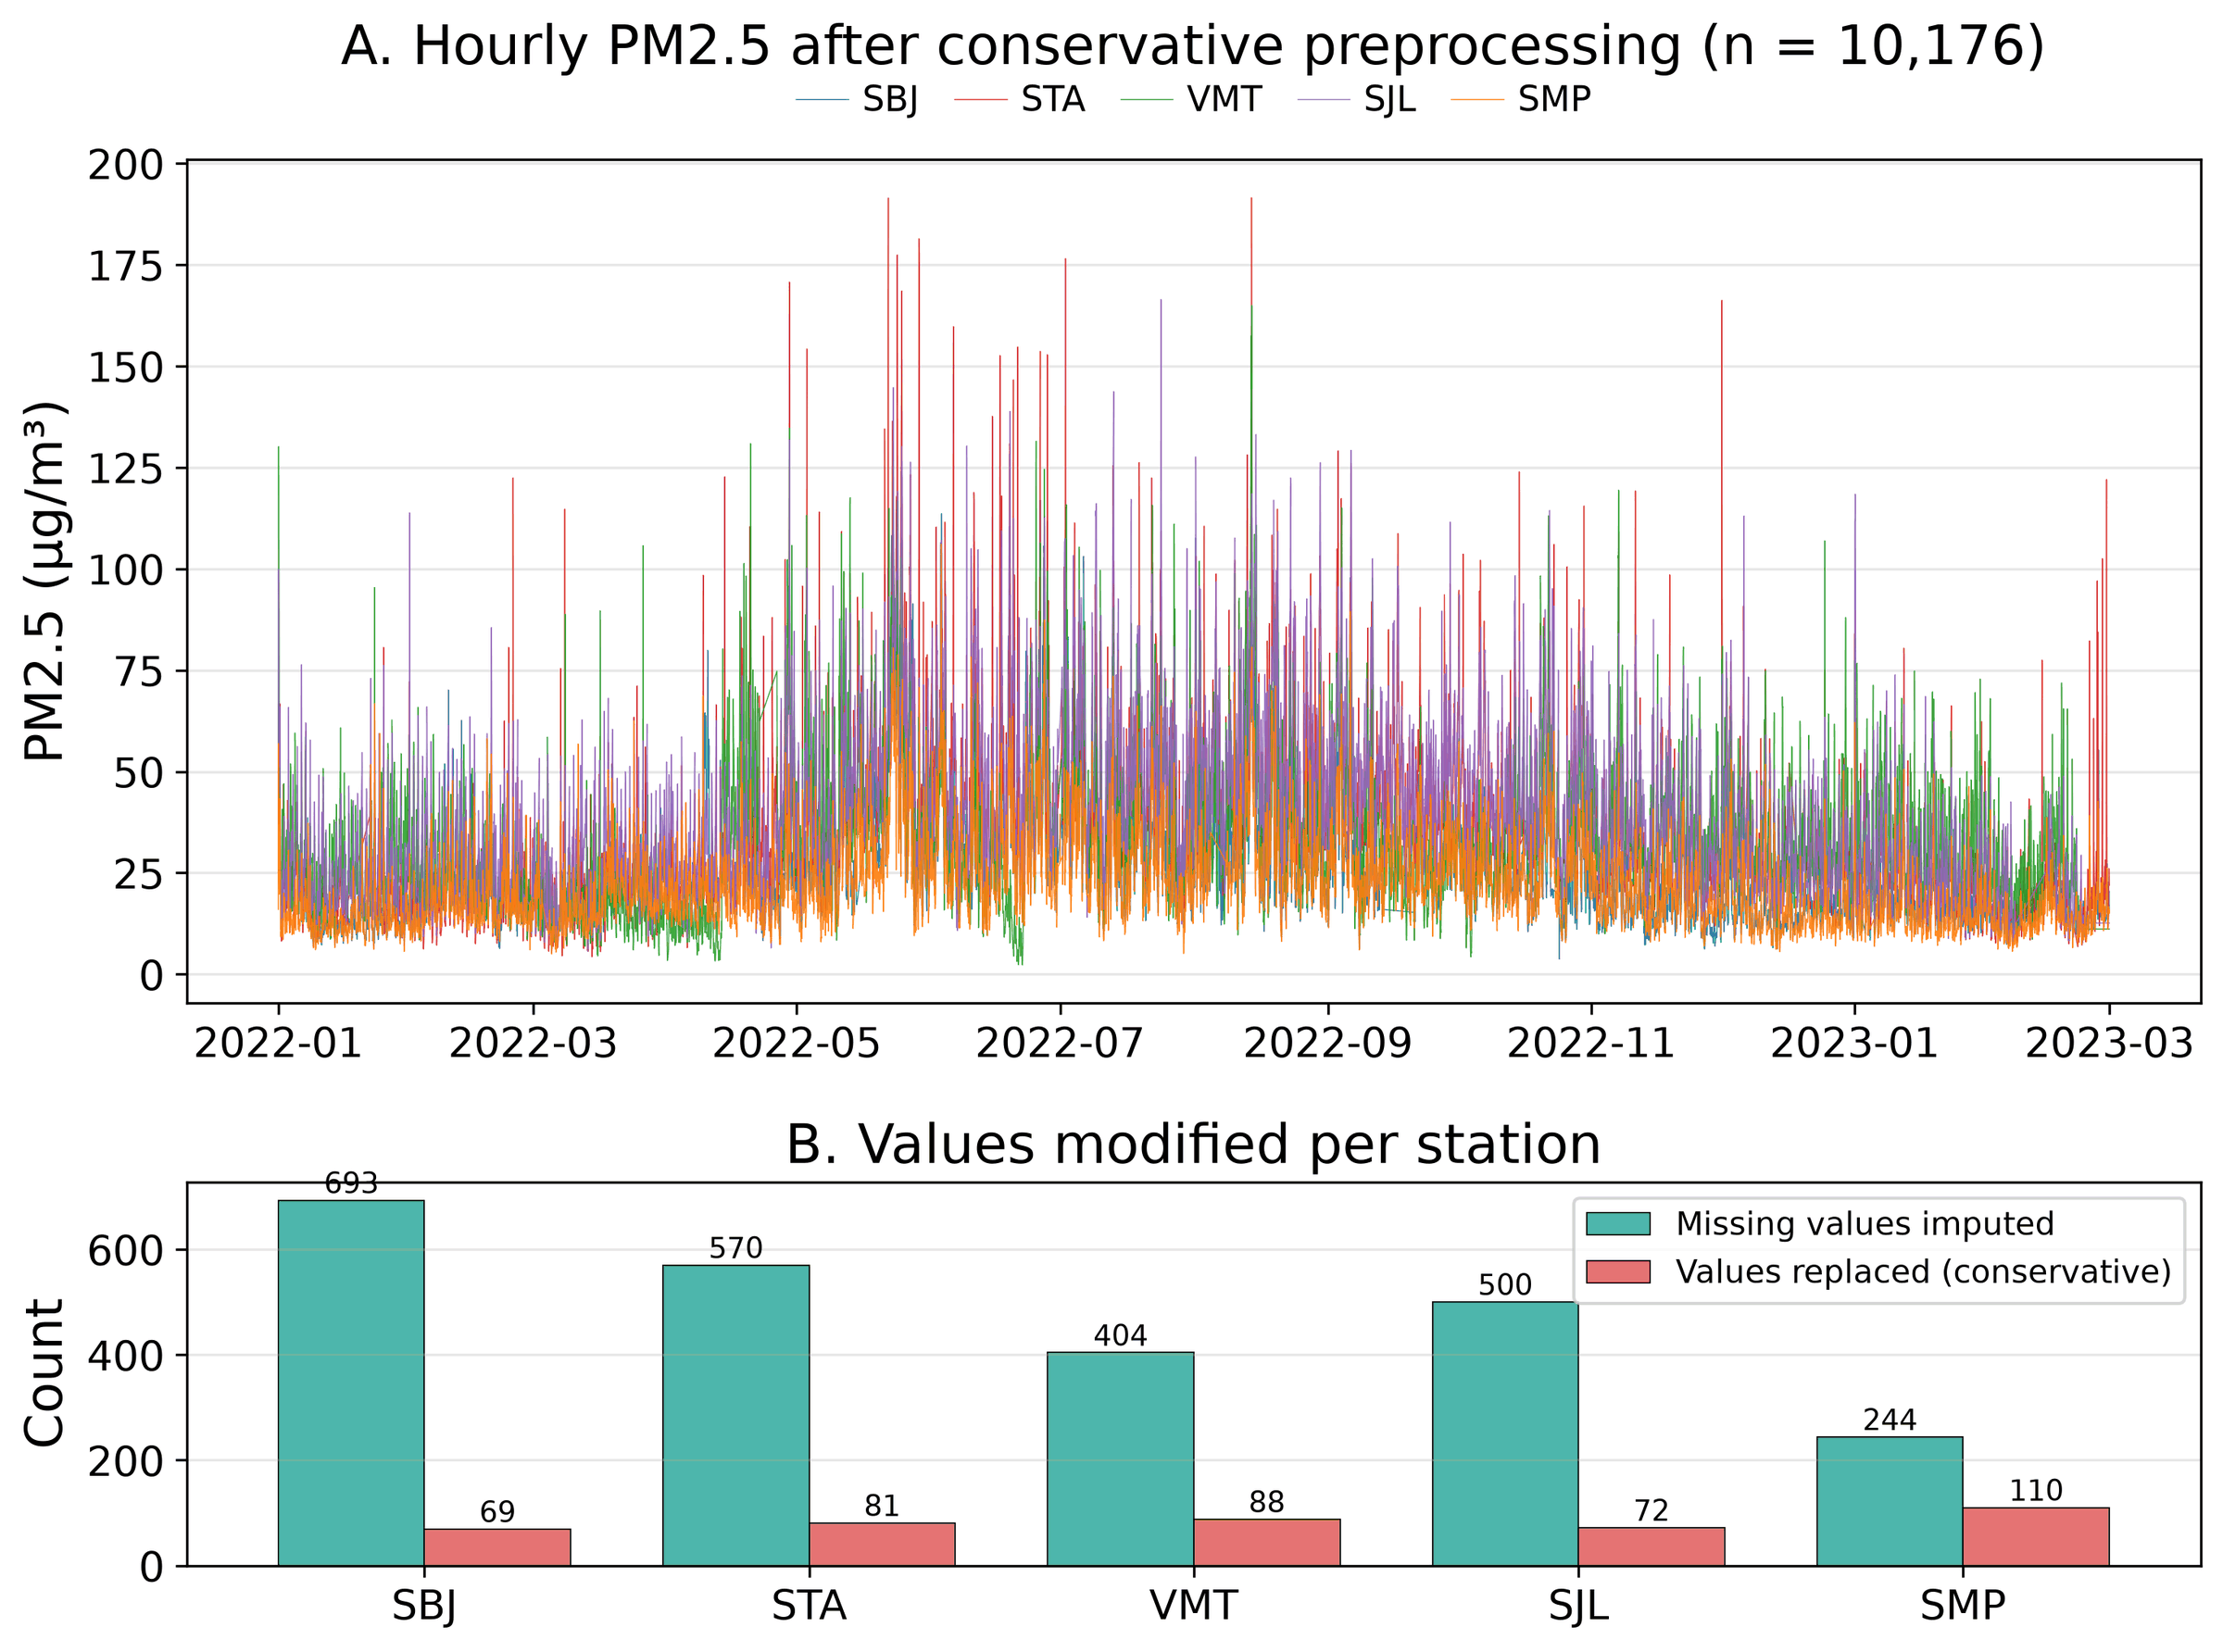
\includegraphics[width=0.80\textwidth,keepaspectratio]{figures/figure_1.png}
\caption{Conservative preprocessing of hourly PM2.5 at five Lima REMCA stations.
\textbf{(A)}~Aligned series ($n=10{,}176$) after imputation and sparse instrumental-error replacement (winter peak June--August 2022; SJL/STA above SBJ/SMP).
\textbf{(B)}~Counts of imputed missing values (teal) and conservatively replaced values (coral). Replacements remain $\sim$0.7--1.1\% of each series.}
\label{fig:preprocessing}
\end{figure}

The city-mean diurnal cycle (Fig.~\ref{fig:diurnal}A) peaks at 09:00 (41.7~$\mu$g\,m$^{-3}$) and troughs at 17:00 (23.8~$\mu$g\,m$^{-3}$). At 09:00, SJL and STA reach 54.9 and 51.6~$\mu$g\,m$^{-3}$, respectively, whereas SBJ and SMP remain near 30~$\mu$g\,m$^{-3}$. Panel~B shows the right-skewed hourly distributions; the WHO 24~h guideline of 50~$\mu$g\,m$^{-3}$ appears only as a reference line, not as an hourly standard. P99 values are 108.4 (STA) and 102.4 (SJL)~$\mu$g\,m$^{-3}$, versus 61.2 at SMP. Pairwise Pearson correlations range from 0.54 (VMT--SMP) to 0.86 (STA--SJL), indicating shared regional forcing modulated by local factors.
\FloatBarrier

\begin{figure}[htbp]
\centering
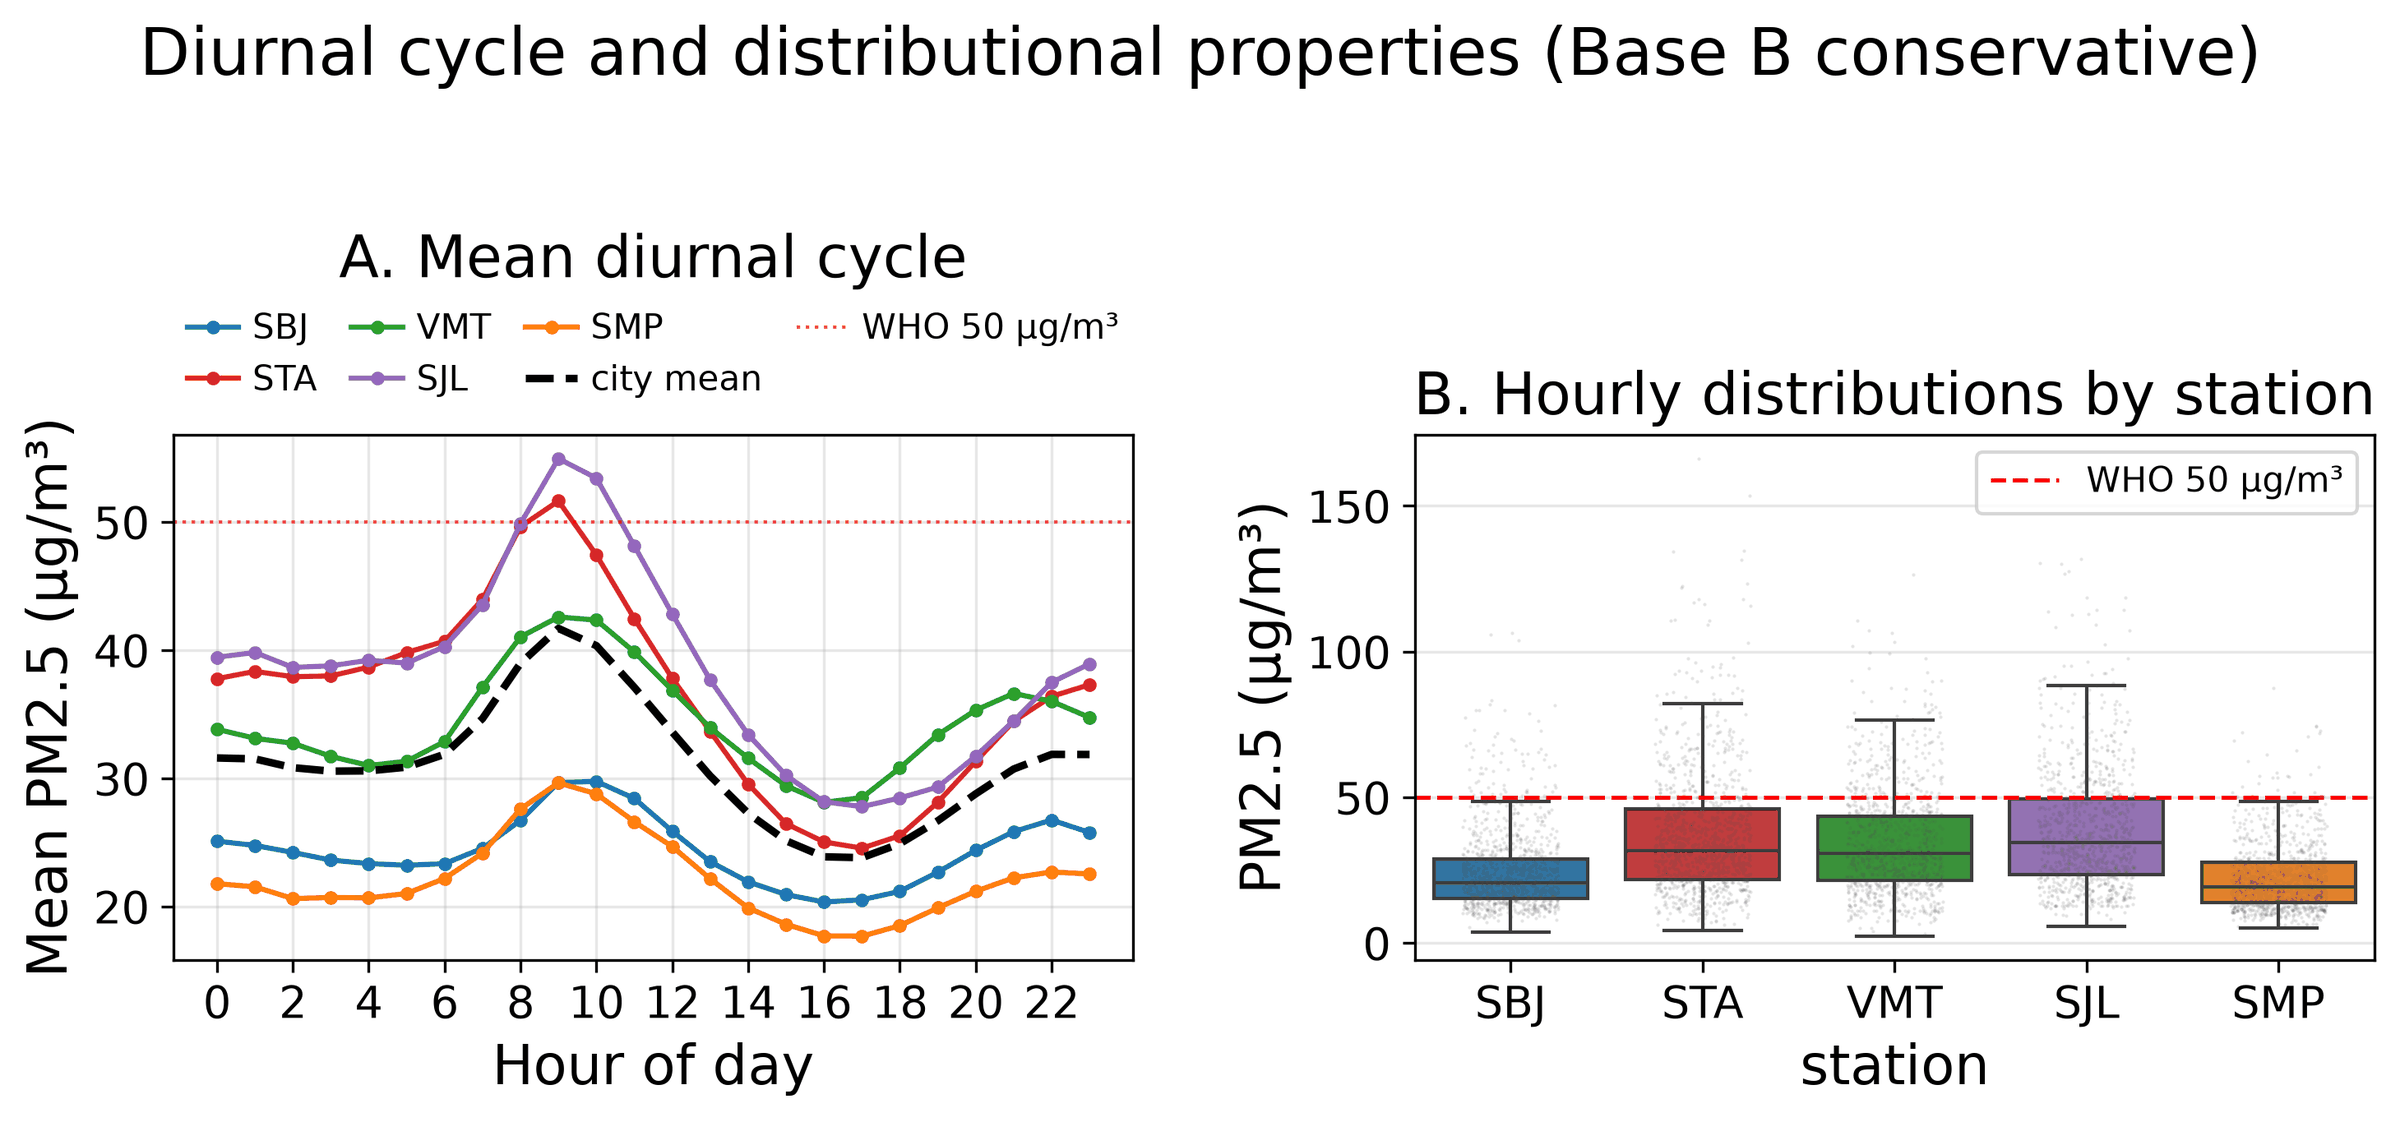
\includegraphics[width=0.80\textwidth,keepaspectratio]{figures/figure_4.png}
\caption{Diurnal cycle and distributions on Base~B.
\textbf{(A)}~Mean hourly concentration by station and city mean (dashed); morning peak at 09:00, afternoon trough at 17:00.
\textbf{(B)}~Hourly distributions; red reference line: WHO 24~h guideline of 50~$\mu$g\,m$^{-3}$.}
\label{fig:diurnal}
\end{figure}

\subsection{Multiscale energy profiles}
\label{subsec:energy}

Figure~\ref{fig:multiscale}A displays $\log_{10}(E_j)$ for $j=1,\ldots,13$. Fine scales ($j=1$--$4$) separate high-energy stations (SJL, STA) from lower-energy sites (SBJ, SMP). In the diurnal band $j=4$, the share of total detail energy is 20.4\% (SJL), 18.7\% (STA), 17.4\% (SMP), 13.3\% (VMT), and 12.4\% (SBJ). Intermediate scales still show separation that shrinks toward longer periods. Grey shading marks levels above the useful DWT maximum; those coarse scales are exploratory only.

\subsection{Scale-wise hypothesis tests}
\label{subsec:hypothesis}

Table~\ref{tab:tests} and Fig.~\ref{fig:multiscale}B summarise assumption-checked tests. Block permutation was required at $j=1$--$4$, 6, and 7 because dependence persisted after aggregation; repeated-measures ANOVA was applied at $j=5$ (independence and normality acceptable); Friedman tests were applied at $j=8$--$9$ (independence acceptable, normality not).

\begin{table}[t]
\centering
\caption{Scale-wise inter-station tests after assumption checking (Base~B). Bonferroni threshold $p<\alpha/9\approx 0.0056$. Effect: Kendall's $W$ or generalised $\eta_G^{2}$.}
\label{tab:tests}
\footnotesize
\setlength{\tabcolsep}{3.5pt}
\begin{tabular}{@{}rllrrrl@{}}
\toprule
$j$ & Period (h) & Method & $p$ & $p_{\mathrm{Bonf}}$ & Sig. & Effect \\
\midrule
1 & 2--4   & Block perm. & $1.0\times10^{-4}$ & $9.0\times10^{-4}$ & Yes & $W{=}0.61$ \\
2 & 4--8   & Block perm. & $1.0\times10^{-4}$ & $9.0\times10^{-4}$ & Yes & $W{=}0.62$ \\
3 & 8--16  & Block perm. & $1.0\times10^{-4}$ & $9.0\times10^{-4}$ & Yes & $W{=}0.65$ \\
4 & 16--32 & Block perm. & $1.0\times10^{-4}$ & $9.0\times10^{-4}$ & Yes & $W{=}0.69$ \\
5 & 32--64 & ANOVA-RM   & $1.4\times10^{-11}$ & $1.3\times10^{-10}$ & Yes & $\eta_G^{2}{=}0.21$ \\
6 & 64--128 & Block perm. & $1.0\times10^{-4}$ & $9.0\times10^{-4}$ & Yes & $W{=}0.35$ \\
7 & 128--256 & Block perm. & $1.0\times10^{-4}$ & $9.0\times10^{-4}$ & Yes & $W{=}0.45$ \\
8 & 256--512 & Friedman & $7.9\times10^{-3}$ & $7.1\times10^{-2}$ & No & $W{=}0.09$ \\
9 & 512--1024 & Friedman & $0.185$ & $1.000$ & No & $W{=}0.08$ \\
\bottomrule
\end{tabular}
\par\vspace{2pt}
\footnotesize Block perm.: block-permutation Friedman; ANOVA-RM: repeated-measures ANOVA; Sig.: significant after Bonferroni correction at $\alpha=0.05$. For block-permutation scales, $p=1.0\times10^{-4}$ is the minimum attainable value, $1/(N_{\mathrm{perm}}+1)$.
\end{table}

\begin{figure}[htbp]
\centering
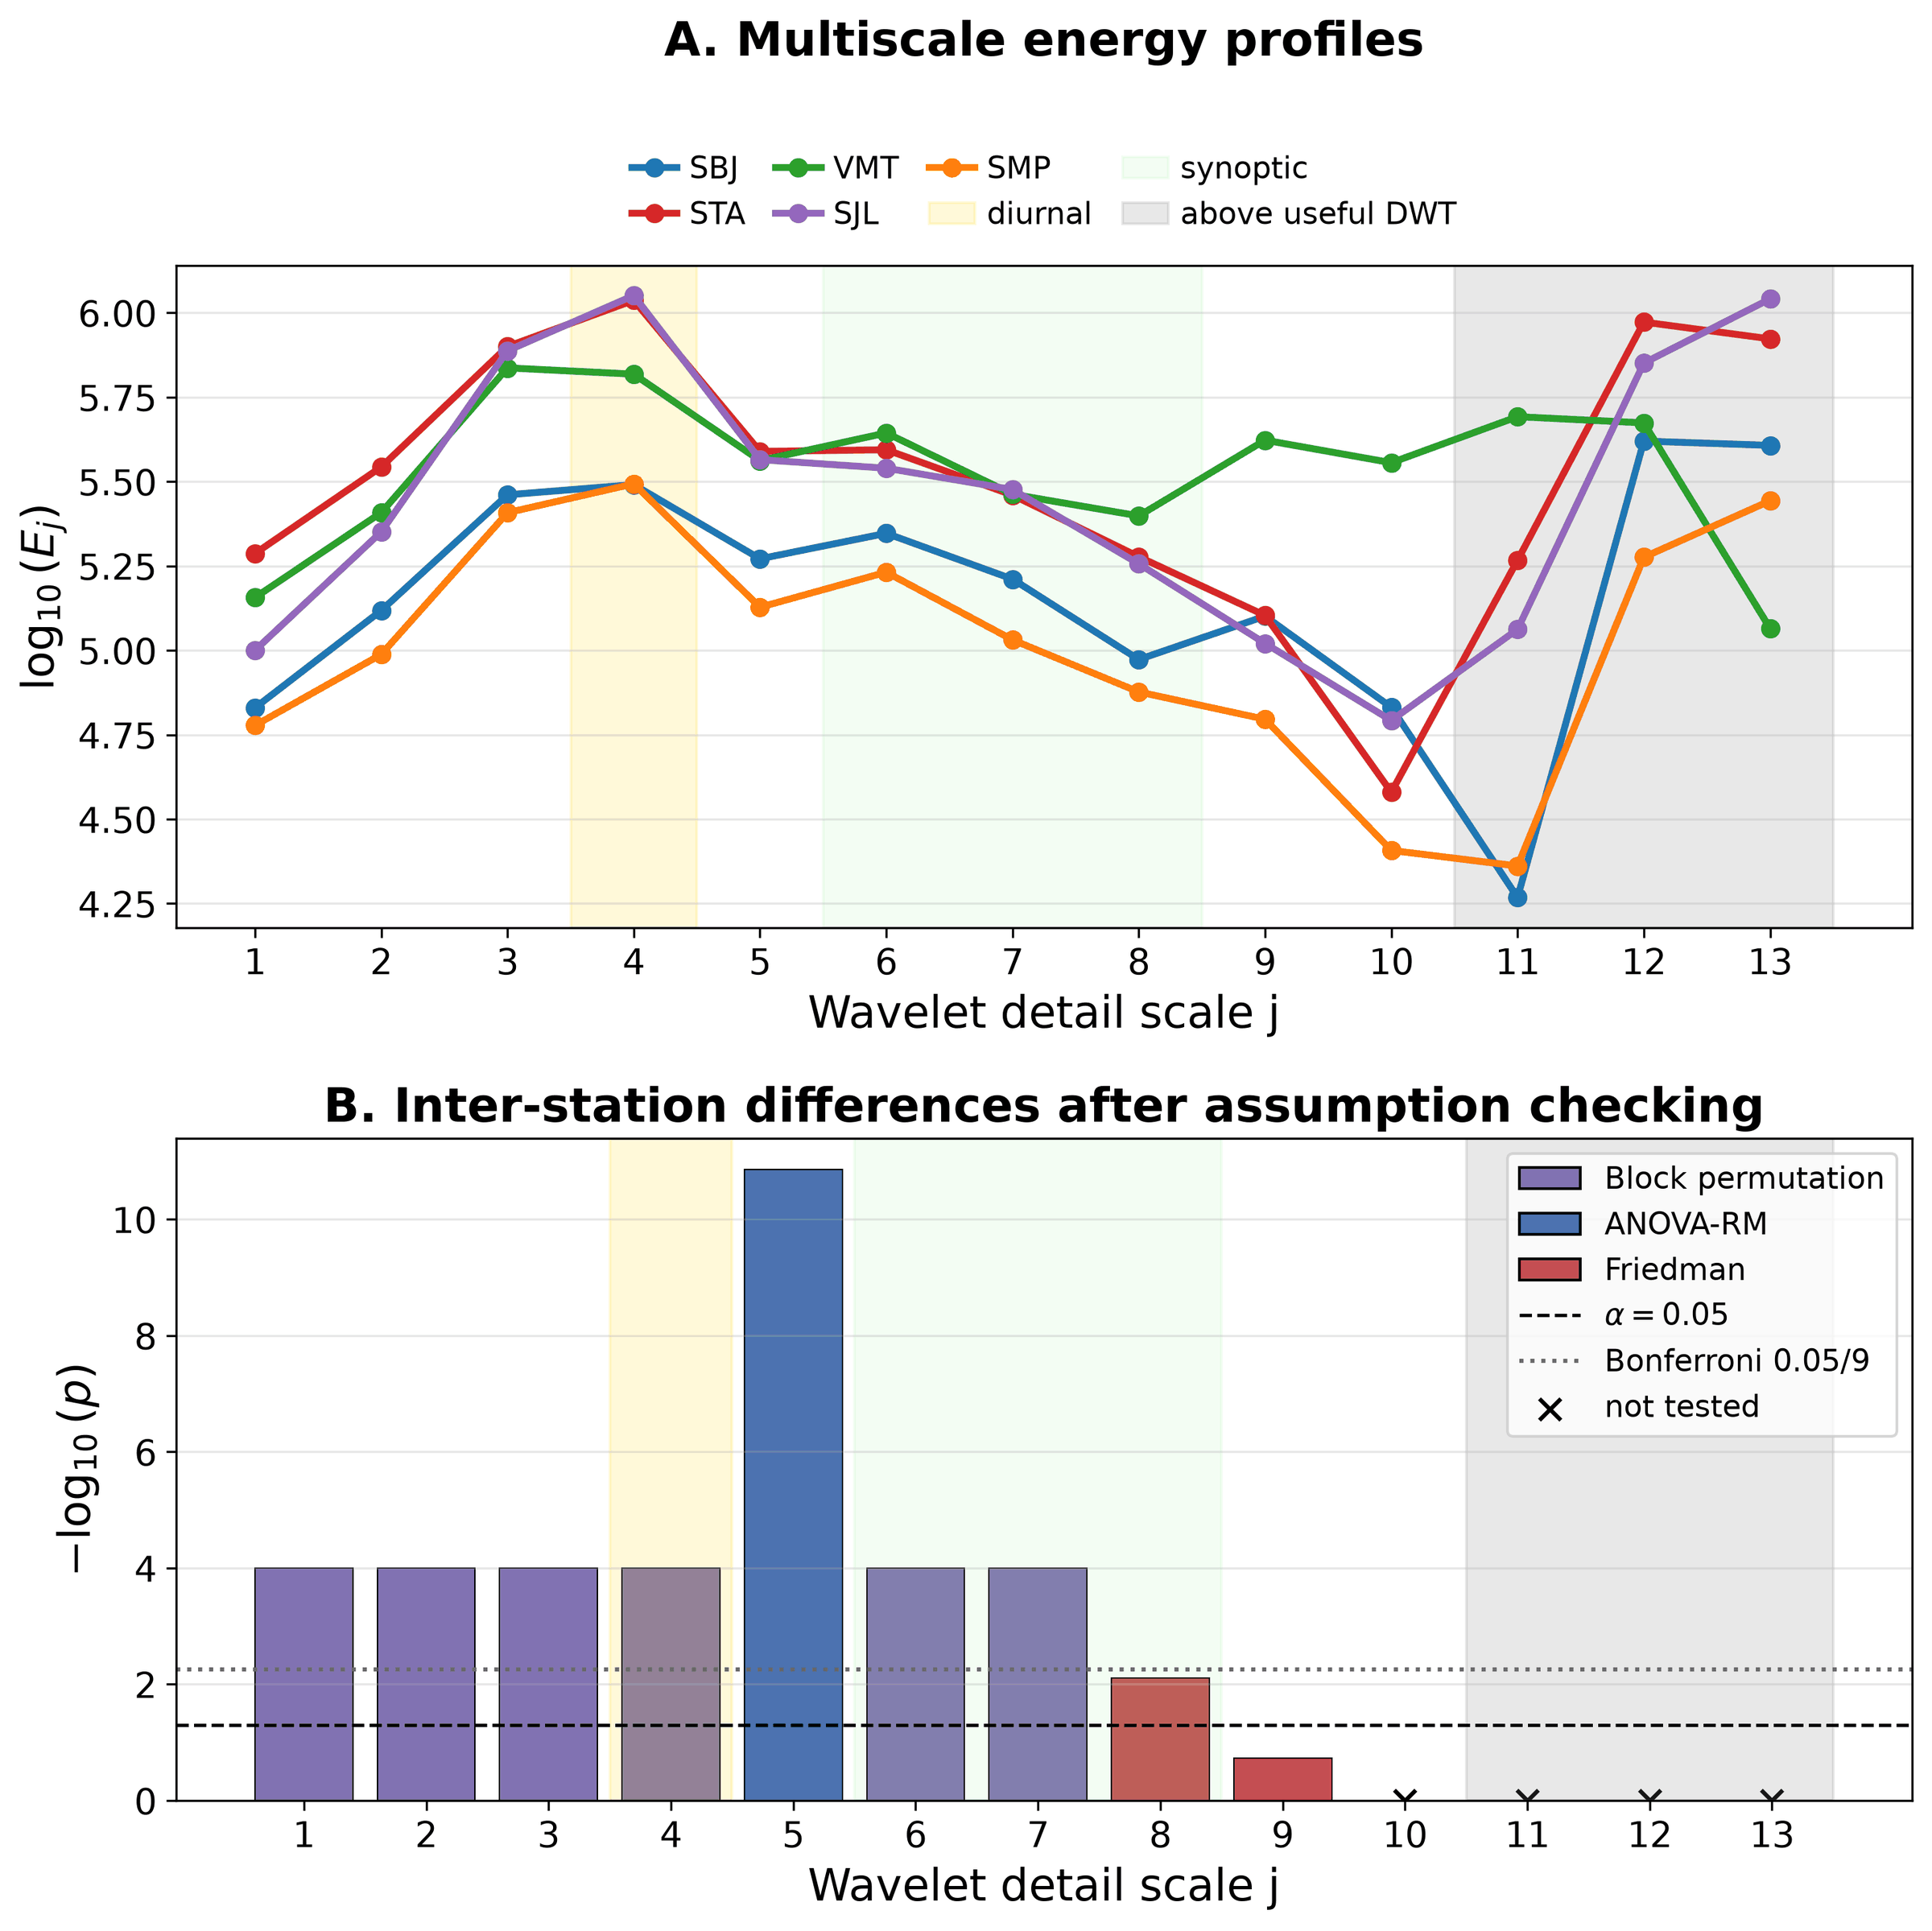
\includegraphics[width=0.80\textwidth,keepaspectratio]{figures/figure_2.png}
\caption{Multiscale energy and assumption-checked inference (Base~B).
\textbf{(A)}~Per-station $\log_{10}(E_j)$ with diurnal (gold) and synoptic (green) bands; grey: above useful DWT level.
\textbf{(B)}~$-\log_{10}(p)$ by selected method (block permutation, ANOVA-RM, or Friedman). Dashed: $\alpha=0.05$; dotted: Bonferroni $0.05/9$; crosses: scales not tested ($j\ge 10$).}
\label{fig:multiscale}
\end{figure}

Bonferroni-significant differences appear at $j=1$--$7$ (about 2~h to $\sim$11 days). For block-permutation scales, the smallest attainable $p$-value with $N_{\mathrm{perm}}=9{,}999$ is $1/(9{,}999+1)=1.0\times10^{-4}$; the table reports this value explicitly rather than as an open inequality. The largest rank-based effect is at $j=4$ ($W=0.69$; 95\% block-bootstrap CI 0.60--0.80). The Friedman test at $j=8$ yielded $p=0.0079$, which does not survive Bonferroni; at $j=9$ there is no evidence of a difference ($p=0.185$). We do not interpret $j\ge 10$ as equality of stations: those scales lack enough central coefficients for reliable formal tests and are influenced by boundary padding. Secondary pairwise Wilcoxon tests (Holm within scale) at $j=1$--$7$ separated the high-contrast corridor stations from the residential sites in most pairs; at $j=4$, eight of ten pairs differed, the exceptions being SJL--STA and SBJ--SMP. These tests are descriptive and do not replace the omnibus Bonferroni decision; pairwise results at $j=8$--$9$ are reported for completeness but not interpreted.

Relative to coefficient-wise Kruskal--Wallis analyses that report extreme $p$-values under independence assumptions, the present $p$-values are more conservative, but the scientific ordering---strong short-scale heterogeneity, weaker intermediate scales, no formal evidence at the longest tested band---is retained. Temporal aggregation produced 19--20 blocks at $j=1$--$7$, 40 at $j=8$, and 20 at $j=9$. These counts are adequate for the omnibus tests but limited for long-scale equivalence claims; the non-significant $j=9$ result is therefore reported as absence of evidence, not as evidence of absence. Sensitivity: Bases A and B share identical Bonferroni decisions; Base C (aggressive) additionally flags $j=8$, illustrating how heavy peak suppression can alter intermediate-scale inference.

\subsection{Diurnal band energy allocation}
\label{subsec:diurnal_energy}

The diurnal band concentrates the strongest rank effect and a clear spatial gradient of energy share (SJL 20.4\%, 95\% CI 17.4--22.9, versus SBJ 12.4\%, 95\% CI 10.3--16.5; the intervals do not overlap), consistent with larger morning peaks at SJL/STA (Fig.~\ref{fig:diurnal}A) and denser traffic corridors. Aggressive cleaning reduces diurnal energy especially at SBJ (to 7.8\%), showing that peak suppression can shrink the very contrast of engineering interest.

\subsection{Interpretation of scale-specific heterogeneity}

Scalar ANOVA on hourly values can establish mean differences but not their timescale. Assumption-checked wavelet tests show that heterogeneity is concentrated from a few hours to about ten days, is strongest in the diurnal band, and loses formal support by $j=9$ ($\sim$21--43 days). This is consistent with a physical partition: local emissions and boundary-layer cycles dominate short scales, whereas basin-wide meteorology increasingly synchronises stations at longer scales. We deliberately avoid claiming that stations are ``indistinguishable'' at seasonal resolutions: those scales were not formally tested with adequate central coefficients.

\subsection{Comparison with previous work}

Functional and multiscale analyses of monitoring networks have been used in Europe and elsewhere to identify representative sites and redesign sparse networks~\cite{ignaccolo2008,gouveia2015}, while wavelet decompositions help separate local events from persistent enhancements in urban sensor systems~\cite{zimmerman2020}. Wavelet-FANOVA theory~\cite{ma2018} has had limited operational use on Latin American air-quality networks. The combination of assumption-checked wavelet inference with an explicit scale-to-objective decision matrix has, to our knowledge, not been reported for a Latin American PM2.5 network. The present study supplies a reproducible pipeline for Lima that ties residual diagnostics to test choice and documents how preprocessing changes multiscale conclusions relevant to network design~\cite{pacsi2016,campos2024}.

\subsection{Practical implications for monitoring networks}

The results support an engineering decision rule. For short-term exposure and diurnal compliance diagnostics, spatial density should be preserved or increased in high-contrast corridors (SJL/STA): morning peaks reach $\approx 55$~$\mu$g\,m$^{-3}$ versus $\approx 30$~$\mu$g\,m$^{-3}$ at SBJ/SMP, and diurnal energy differs by about eight percentage points. For multi-week or basin-scale tracking, the evidence for station-specific differences weakens; a smaller representative subset may be adequate, but this should be tested against the specific objective. Operationally, dense, reliable sampling should be prioritised where $j=1$--$4$ contrasts are large, and weak multi-week differences should not be read as evidence that stations are interchangeable for acute management. Table~\ref{tab:decision} summarises these implications by monitoring objective.

\begin{table}[htbp]
\centering
\caption{Evidence-based decision matrix for monitoring effort. Timescales follow the DWT bands of Table~\ref{tab:tests}; recommendations are conditional on the five-station, 14-month evidence base.}
\label{tab:decision}
\footnotesize
\setlength{\tabcolsep}{3pt}
\begin{tabularx}{\textwidth}{@{}>{\raggedright\arraybackslash}p{3.0cm}>{\raggedright\arraybackslash}p{2.4cm}>{\raggedright\arraybackslash}X>{\raggedright\arraybackslash}p{4.2cm}@{}}
\toprule
Monitoring objective & Relevant scales & Evidence & Implication \\
\midrule
Acute and diurnal exposure & $j=1$--$4$ (2--32~h) & Strongest inter-station differences; $W$ up to 0.69; 09:00 peaks $\approx$55 versus $\approx$30~$\mu$g\,m$^{-3}$ (SJL/STA versus SBJ/SMP) & Preserve hourly resolution and prioritise short-scale coverage in high-contrast corridors \\
Synoptic and weekly tracking & $j=5$--$7$ (32~h--11~d) & Bonferroni-significant but weaker effects ($W=0.35$--$0.45$; $\eta_G^2=0.21$) & Retain spatial coverage; interpret station-specific weekly anomalies cautiously \\
Multi-week and seasonal & $j=8$--$9$ (10--43~d) & No Bonferroni evidence; $j=9$ has low power (20 blocks) & Do not infer station redundancy; use dedicated seasonal or trend analyses \\
Long-term trends & $j\ge10$ & Not formally testable with this series length & Use a separate trend model; not a basis for network reduction \\
\bottomrule
\end{tabularx}
\end{table}

\subsection{Methodological considerations}

Conservative preprocessing addresses right-skewed PM2.5 tails: only 0.7--1.1\% of hours are replaced, and sensitivity shows complete Bonferroni agreement between imputation-only and conservative bases. Adaptive tests address dependence that classical Kruskal--Wallis on all $d_{j,k}^{2}$ ignores. Several limitations remain. The record covers five stations and 14 months, so the decision matrix is a case-specific engineering input rather than a universal design rule. One long curve per station limits the number of independent replicates; Hampel and medcouple thresholds were fixed a priori; and coarse scales are affected by boundary padding. No meteorological covariates or source apportionment are used, so the physical interpretation identifies plausible mechanisms rather than attributing sources. The former aggressive 8--13\% replacement rule is retained only as a contrast arm, not as the primary scientific analysis.


% =============================================================================
\section{Conclusions}
\label{sec:conclusions}
% =============================================================================

For Lima REMCA hourly PM2.5 (Base~B), inter-station differences are Bonferroni-significant at scales $j=1$--$7$, strongest at the diurnal band ($j=4$, Kendall's $W=0.69$, 95\% CI 0.60--0.80), not Bonferroni-significant at $j=8$, and non-significant at $j=9$; $j\ge10$ cannot be tested formally with this record length. Diurnal energy fractions range from 12.4\% (SBJ) to 20.4\% (SJL).

Conservative cleaning replaces fewer than about 1.1\% of hours; sensitivity to imputation-only data leaves the main significance pattern unchanged, whereas aggressive STL+$3\times$IQR can alter intermediate-scale calls. The resulting decision matrix supports denser short-scale monitoring in high-contrast corridors and cautions against inferring multi-week redundancy. These conclusions are conditional on five stations and a 14-month record; extending the framework to other networks should revisit the preprocessing and block structure.

% =============================================================================
\section*{Declaration of Competing Interest}
The authors declare that they have no known competing financial interests or personal relationships that could have appeared to influence the work reported in this paper.

\section*{Acknowledgments}
The authors thank SENAMHI for REMCA open data and continuous network operations.

\section*{Funding}
The authors received no specific external funding for this research.

\section*{Authors' Contributions}
H.S.~Aquino-Mosquera: Conceptualization, Methodology, Software, Formal analysis, Writing---original draft.
J.E.~Villanueva-Ram\'irez: Data curation, Validation, Writing---review \& editing.
D.A.~Huam\'an-C\'ardenas: Formal analysis, Software, Visualization.
G.R.~Quispe-Mendoza: Supervision, Investigation, Writing---review \& editing.

\section*{Data Availability Statement}
Hourly PM2.5 data are publicly available from SENAMHI REMCA (\url{https://www.senamhi.gob.pe}).
\begin{sloppypar}
Processed bases, the row-level preprocessing audit, analysis scripts, configuration files and figure sources are available at \url{https://github.com/jelincovil/pm25-lima-wavelet} (release v1.0.2). A DOI will be minted for the archived release.
\end{sloppypar}

\noindent Corresponding author: Henry S. Aquino-Mosquera (\url{henry.aquino@ciencia.org.pe}).

% =============================================================================
\begin{thebibliography}{21}

\bibitem{watts2018}
N.~Watts \textit{et al.},
``The Lancet Countdown on health and climate change: From 25 years of inaction to a global transformation for public health,''
\textit{The Lancet}, vol.~391, no.~10120, pp.~581--630, 2018.

\bibitem{iqair2023}
IQAir, ``2023 World Air Quality Report,'' 2024. [Online].
Available: \url{https://www.iqair.com/world-air-quality-report}

\bibitem{pacsi2016}
S.~A. Pacsi Valdivia,
``An\'alisis temporal y espacial de la calidad del aire determinado por material particulado PM10 y PM2,5 en Lima Metropolitana,''
\textit{Anales Cient\'ificos}, vol.~77, no.~2, pp.~273--283, 2016, doi: 10.21704/ac.v77i2.699.

\bibitem{campos2024}
A.~H. Campos D\'iaz \textit{et al.},
``A spatio-temporal behavior of PM2.5 and PM10 on changes of their concentration levels in the metropolitan area of Lima,''
\textit{Int.\ J.\ Sustain.\ Dev.\ Plan.}, vol.~19, no.~10, pp.~4083--4092, 2024, doi: 10.18280/ijsdp.191036.

\bibitem{vu2019}
B.~N. Vu \textit{et al.},
``Developing an advanced PM2.5 exposure model in Lima, Peru,''
\textit{Remote Sens.}, vol.~11, no.~6, p.~641, 2019, doi: 10.3390/rs11060641.

\bibitem{who2021}
World Health Organization,
\textit{WHO Global Air Quality Guidelines: Particulate Matter (PM2.5 and PM10), Ozone, Nitrogen Dioxide, Sulfur Dioxide and Carbon Monoxide}.
Geneva, Switzerland: WHO, 2021.

\bibitem{romerobaylon2024}
A.~A. Romero-Bayl\'on \textit{et al.},
``Spatial localization of air pollutants in Lima: Air quality monitoring in the troposphere,''
\textit{Int.\ J.\ Environ.\ Impacts}, vol.~7, no.~3, pp.~485--493, 2024, doi: 10.18280/ijei.070310.

\bibitem{morettin2017}
P.~Morettin,
``Wavelets in functional data analysis,''
\textit{International Statistical Review}, vol.~85, no.~2, pp.~202--226, 2017.

\bibitem{ignaccolo2008}
R.~Ignaccolo, S.~Ghigo, and E.~Giovenali,
``Analysis of air quality monitoring networks by functional clustering,''
\textit{Environmetrics}, vol.~19, no.~7, pp.~672--686, 2008, doi: 10.1002/env.946.

\bibitem{cardot1999}
H.~Cardot, F.~Ferraty, and P.~Sarda,
``Functional linear model,''
\textit{Statistics \& Probability Letters}, vol.~45, no.~1, pp.~11--22, 1999.

\bibitem{hall2007}
P.~Hall and J.~L. Horowitz,
``Methodology and convergence rates for functional linear regression,''
\textit{Annals of Statistics}, vol.~35, no.~1, pp.~70--91, 2007.

\bibitem{abramovich2000}
F.~Abramovich, T.~Bailey, and T.~Sapatinas,
``Wavelet analysis and its statistical applications,''
\textit{The Statistician}, vol.~49, no.~1, pp.~1--29, 2000.

\bibitem{antoniadis2007}
A.~Antoniadis,
``Wavelet methods in statistics: Some recent developments and their applications,''
\textit{Statistics Surveys}, vol.~1, pp.~16--55, 2007.

\bibitem{gouveia2015}
S.~Gouveia, M.~G. Scotto, A.~Monteiro, and A.~M. Alonso,
``Wavelets-based clustering of air quality monitoring sites,''
\textit{Environ.\ Monit.\ Assess.}, vol.~187, no.~11, p.~694, 2015, doi: 10.1007/s10661-015-4911-x.

\bibitem{zimmerman2020}
N.~Zimmerman \textit{et al.},
``Improving correlations between land use and air pollutant concentrations using wavelet analysis: Insights from a low-cost sensor network,''
\textit{Aerosol Air Qual.\ Res.}, vol.~20, pp.~314--328, 2020, doi: 10.4209/aaqr.2019.03.0124.

\bibitem{abramovich2006}
F.~Abramovich and Y.~Benjamini,
``Thresholding of wavelet coefficients as multiple hypotheses testing procedure,''
in \textit{Wavelets and Statistics}, A.~Antoniadis and G.~Oppenheim, Eds.
New York: Springer, 2006, pp.~5--14.

\bibitem{ma2018}
L.~Ma and J.~Soriano,
``Efficient functional ANOVA through wavelet-domain Markov groves,''
\textit{Journal of the American Statistical Association}, vol.~113, no.~522, pp.~802--818, 2018.

\bibitem{cleveland1990}
R.~B. Cleveland, W.~S. Cleveland, J.~E. McRae, and I.~Terpenning,
``STL: A seasonal-trend decomposition procedure based on loess,''
\textit{Journal of Official Statistics}, vol.~6, no.~1, pp.~3--73, 1990.

\bibitem{daubechies1992}
I.~Daubechies,
\textit{Ten Lectures on Wavelets}.
Philadelphia, PA, USA: SIAM, 1992, doi: 10.1137/1.9781611970104.

\bibitem{mallat1989}
S.~G. Mallat,
``A theory for multiresolution signal decomposition: The wavelet representation,''
\textit{IEEE Trans.\ Pattern Anal.\ Mach.\ Intell.}, vol.~11, no.~7, pp.~674--693, 1989, doi: 10.1109/34.192463.

\bibitem{nason2008}
G.~P. Nason,
\textit{Wavelet Methods in Statistics with R}.
New York, NY, USA: Springer, 2008, doi: 10.1007/978-0-387-75962-3.

\end{thebibliography}

\end{document}
